\section{Lattice Boltzmann Models}
\label{LBS}

\paragraph{}Lattice Boltzmann models (LBM) is a class of computational fluid dynamics (CFD) methods for fluid simulation. Instead of solving the Navier–Stokes equations, the discrete Boltzmann equation is solved to simulate the flow of a Newtonian fluid with collision models such as Bhatnagar-Gross-Krook (BGK). By simulating streaming and collision processes across a limited number of particles, the intrinsic particle interactions create a flow behavior applicable across an entire lattice.

\paragraph{}Lattice Gas Cellular Automaton (LGCA) models were the harbingers of LBM. LGCA were presented as a viable means of solving the Navier-Stokes equations of fluid motion. Ludwig Boltzmann used these models to introduce the Boltzmann Gas Concept, where the idea is that a gas is composed of interacting particles that can be described by classical mechanics, and, because there are so many particles, a statistical treatment is necessary and appropriate. The mechanics can be extremely simple and encapsulated by just
the notions of streaming in space and billiard-like collision interactions.

\paragraph{}LBM vastly simplify Boltzmann’s original conceptual view by reducing the number of possible particle spatial positions and microscopic momenta from a continuum to just a handful and similarly discretizing time into distinct steps. Particle positions are confined to the nodes of the lattice. Variations in momenta that could have been due to a continuum of velocity directions and magnitudes and varying particle mass are reduced, in the simple 2-D model, to 8 microscopic velocity directions, and a single particle mass \citep{sukop2006lattice}. 

\paragraph{}Using these microscopic velocities, we can obtain a macroscopic velocity, which is the one that dictates the flow within a lattice. \fref{fig:d2q9} shows the Cartesian lattice and the velocities $e_a$ where a = 0, 1, \dots , 8 is a direction index and $e_0$ = 0 denotes particles at rest. This model is known as D2Q9 as it is 2 dimensional and contains 9 velocities. The lattice unit (lu) is the fundamental measure of length in the LBM models and time steps (ts) are the time unit. 

\paragraph{}Other fundamental element of the LBM is the single-particle distribution function $f$. The distribution function can be thought of as a typical histogram representing a frequency of occurrence. The frequencies can be considered to be direction-specific fluid densities.

\begin{figure}[t]
    \centering
    \begin{subfigure}[t!]{0.45\textwidth}
        \centering
        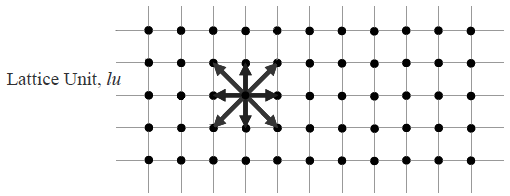
\includegraphics[scale=0.7]{d2q9.png}
        \caption{A sample 2D Lattice. The dots represent the nodes of the lattice.}
        \label{fig:2Dlattice}
    \end{subfigure}
	\hfill
    \begin{subfigure}[t!]{0.45\textwidth}
        \centering
        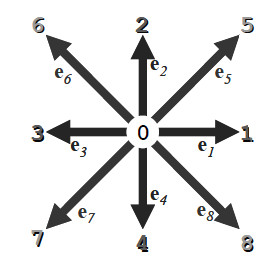
\includegraphics[scale = 0.7]{LatticeElement.png}
        \caption{Each Lattice node has 8 possible velocity directions. }
        \label{fig:latticeElement}
    \end{subfigure}

    \caption{D2Q9 lattice. Adapted from \citep{sukop2006lattice}.}
    \label{fig:d2q9}
\end{figure}

\paragraph{}These models can also be implemented in three dimensions. The main difference with the two dimension models are the amount of velocities and their directions. There are several possibilities, from models that use twenty seven direction, to models that use only thirteen. However, the most used model is the one that has nineteen velocities, the d3q19 model, because it yields the best equilibrium between precision and used memory \citep{rinaldi2011modelos}. 

\subsection{Lattice Boltzmann Solver}

\paragraph{}In order to develop a LBM solver, we have to take into account the basic parts and equations that define the models. These are:

\begin{itemize}
	\item Streaming: Each node's distribution function is updated in relation to the other nodes in the lattice. Specifically, the direction-specific densities $f_a$ to the nearest neighbor lattice nodes. The streaming equation is as follows:
	\begin{equation}
		f_a(x + e_a \Delta t, t + \Delta t) = f_a(x,t)
	\end{equation}
	where $x$ is the lattice node position, $e_a$ is the direction index, $t$ is the time step, and $\Delta t$ is the next step in the simulation.
	\item Collision: Collision of the fluid particles is considered as a relaxation towards a local equilibrium. The collision equations are as follows:
	\begin{equation}
		f_a(x,t) = f_a(x,t) - \frac{f_a(x,t)-f_a^{eq}(x,t)}{\tau}
	\end{equation}
	where $f_a^{eq}$ is the equilibrium function, and $\tau$ is a relaxation parameter that controls the fluid viscosity. The equilibrium function is defined as:
	\begin{equation}
		f_a^{eq}(x,t) = w_a \rho(x)[1 + \frac{e_a \cdot u}{c^2} + \frac{(e_a \cdot u)^2}{2 c^4} - \frac{u^2}{2 c^2}]
	\end{equation}
	where $w_a$ are weights corresponding to each lattice velocity, $\rho$ is the macroscopic density, and $c$ is the basic speed of the lattice.
	\item Boundary Condition: We have to take into account the boundaries of the lattice since the nodes situated at the edges have no neighbor cells from which to obtain a distribution in the streaming step. We can also incorporate solid boundaries in the models, in order to simulate realistic porous media, for example.
\end{itemize} 

\paragraph{}For more details on the formulation of LBM and its equations, refer to \citep{sukop2006lattice, rinaldi2011modelos} and the references mentioned within.

\paragraph{}We have implemented the d3q19 model using the CUDA API. Since we want to simulate biological tissue, normal boundary conditions do not apply; we only need the solid boundary conditions. We surrounded the lattice with solid elements, which serve as a container, in order to get the fluid to "flow" inside said container. 

\paragraph{}\fref{fig:lb_cuda} shows a sample lattice were the the macroscopic velocities are displayed. To better represent the flow within the sample lattice, we induced the flow by defining a direction vector, and applying it at a determinate point of the lattice. We created a cube within the lattice in order for the macroscopic velocities to move around said cube. \fref{fig:lb_cuda_noflow} shows a different lattice, where no flow direction vector is added. We found that this lattice is in an equilibrium state, and all the macroscopic velocities flow toward the outside of the lattice. This is a property of the LBM that will enable us to create tissues that are able to preserve their volume.

\begin{figure}[t]
    \centering
    \begin{subfigure}[h]{0.45\textwidth}
        \centering
    		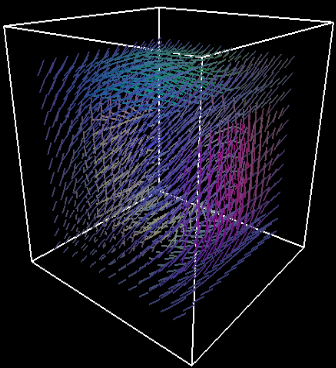
\includegraphics[scale=0.7]{lb_cuda.png}
    		\caption{A 3D lattice with an external flow.}
    		\label{fig:lb_cuda}
    \end{subfigure}
	\hfill
    \begin{subfigure}[h]{0.45\textwidth}
        \centering
        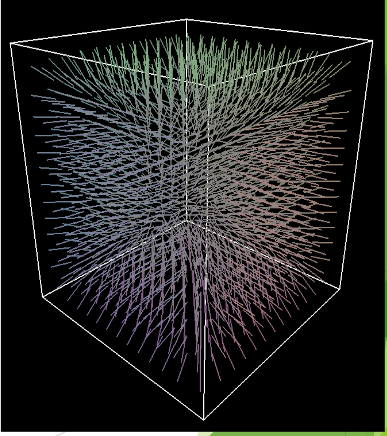
\includegraphics[scale = 0.6]{lb_cuda_noflow.png}
        \caption{A 3D lattice without an external flow.}
        \label{fig:lb_cuda_noflow}
    \end{subfigure}

    \caption{Implementation of the 3D Lattice Boltzmann method using CUDA.}
    \label{fig:d3q19}
\end{figure}

\subsection{Solver details and results}

\paragraph{}We tested two different approaches for the CUDA implementation of the Lattice Boltzmann Solver. The first approach was using Thrust. Thrust is a C++ template library for CUDA based on the Standard Template Library (STL). It allows the implementation of high performance parallel applications with minimal programming effort through a high-level interface that is fully interoperable with CUDA C \citep{nvidia2015thrust}. Using thrust the development of the solver was straightforward. After a CPU version was developed, we used the \textit{thrust::for\_each} algorithm to map the different steps of the solver to each lattice node using different kernels.

\paragraph{} The second approach was using the CUDA API directly. For that approach, we designed two main kernels, one for the streaming and one for the collide steps. Both kernels use global memory, and are configured using a bi dimensional array of blocks defined by the lattice width and height, and a bi dimensional array of threads. We varied the size of the thread array to try to obtain optimal execution times. For the collision step, we found that using fixed block and thread sizes we obtained the best results. We used a bi dimensional array of blocks defined by the lattice width and height, and a number of threads equal to the lattice depth. 

\paragraph{}In order to test the performance of our solution, we limited a simulation to a thousand iterations of the solver, and we measured the execution times of the streaming and collide steps for different grid sizes. We also measured the the performance in terms of Million Lattices Updates Ser Second (MLUPS) and GPU/CPU speedup. Here, the MLUPS is given by:

\begin{equation}
	MLUPS = \frac{grid Size * 10^{-6}}{iteration time (s)}
\end{equation}

\paragraph{}Table \ref{tab:lbm_cpu} shows the average times of a simulation of the solver in CPU. 

\begin{table}[htbp]
  \centering
    \begin{tabular}{|c|c|c|c|c|}
    \toprule
    \multicolumn{5}{c}{\textbf{LBM using CPU}} \\
    \midrule
    \textbf{Lattice Size	} & \textbf{Stream Avg (ms)} &	 \textbf{Collide Avg (ms)} & \textbf{Total Avg (ms)} & \textbf{MLUPS Avg} \\ 
    30x30x30 & 	2.5697	 & 4.2447& 6.8145& 3.9995\\
    50x50x50&	12.5627&	21.4232&33.9860&3.6944\\
	100x100x100&110.4029&198.6268&309.0298&	3.2368\\
	132x132x132&	258.7472&464.9450&723.6923&3.1783\\
    \bottomrule
    \end{tabular}%
    \caption{LBM simulation times using the CPU.}
  \label{tab:lbm_cpu}%
\end{table}%

\paragraph{}Based on the times obtained using just the CPU, in Table \ref{tab:lbm_gpu_thrust} we present the average times, speedup, and MLUPS for a simulation using CUDA THRUST. As it will be seen in the following tables, the thrust implementation yielded good results, but as we give up a certain amount of control, we can not control the simulation as much as needed to improve performance.

\begin{table}[htbp]
  \centering
    \begin{tabular}{|c|c|c|c|c|c|}
    \toprule
    \multicolumn{6}{c}{\textbf{LBM using GPU, CUDA THRUST}} \\
    \midrule
    \textbf{Lattice Size	} & \textbf{Stream Avg (ms)} &	\textbf{ Collide Avg (ms)} & \textbf{Total Avg (ms)} & \textbf{MLUPS Avg} &\textbf{Speedup}\\
    30x30x30	&0.2751 &	3.9406 	&4.2158 	&6.4045 	&1.6164 \\
50x50x50&	1.2667 &	17.1502 	&18.4169 &	1.4686 &	1.8453 \\
100x100x100&	12.5523 	&135.9719 &	148.5243&	6.7342 &	2.0806  \\

    \bottomrule
    \end{tabular}%
       \caption{LBM simulation times using the GPU and the CUDA Thrust template library.}
  \label{tab:lbm_gpu_thrust}%
\end{table}%

\paragraph{}In Table \ref{tab:lbm_gpu_8} we present the average times, speedup, and MLUPS for a simulation using an array of 8 by 19 threads for the streaming step. Table \ref{tab:lbm_gpu_53} shows the results for  an array of 53 by 19 threads.

%\begin{table}[htbp]
%  \centering
%    \begin{tabular}{|c|c|c|c|c|c|}
%    \toprule
%    \multicolumn{6}{c}{\textbf{LBM using GPU, 4 Threads}} \\
%    \midrule
%    \textbf{Lattice Size	} & \textbf{Stream Avg (ms)} &	\textbf{ Collide Avg (ms)} & \textbf{Total Avg (ms)} & \textbf{MLUPS Avg} &\textbf{Speedup}\\
%    30x30x30	&0.1633&0.6448&0.8082&	33.4457&	8.4315\\
%	50x50x50	&1.0837&2.6658&3.7496	&33.4456&9.0637\\
%	132x132x132&	30.9862&	89.3489&	120.3352&	19.1142&6.0139\\
%    \bottomrule
%    \end{tabular}%
%     \caption{LBM simulation times using the GPU and an array of 4 by 19 threads to calculate the streaming step.}
%  \label{tab:lbm_gpu_4}%
%\end{table}%

\begin{table}[htbp]
  \centering
    \begin{tabular}{|c|c|c|c|c|c|}
    \toprule
    \multicolumn{6}{c}{\textbf{LBM using GPU, 8 Threads}} \\
    \midrule
    \textbf{Lattice Size	} & \textbf{Stream Avg (ms)} &	\textbf{ Collide Avg (ms)} & \textbf{Total Avg (ms)} & \textbf{MLUPS Avg} &\textbf{Speedup}\\
    30x30x30	&0.1984&0.6624&0.8609&31.3618&	7.9151\\
	50x50x50&	1.1635&	2.7446&	3.9081&31.9848&8.6961\\
	132x132x132	&27.3471&86.4619&	113.8091&20.2109&6.3588\\
    \bottomrule
    \end{tabular}%
	\caption{LBM simulation times using the GPU and an array of 8 by 19 threads to calculate the streaming step.}
	\label{tab:lbm_gpu_8}%
\end{table}%

\begin{table}[htbp]
  \centering
    \begin{tabular}{|c|c|c|c|c|c|}
    \toprule
    \multicolumn{6}{c}{\textbf{LBM using GPU, 53 Threads}} \\
    \midrule
    \textbf{Lattice Size	} & \textbf{Stream Avg (ms)} &	\textbf{ Collide Avg (ms)} & \textbf{Total Avg (ms)} & \textbf{MLUPS Avg} &\textbf{Speedup}\\
    30x30x30&	0.4269	&0.6627&1.0896&24.7784&6.2536\\
50x50x50&	1.714 	&2.6427 	&4.3570	&28.7034 &	7.8001\\
132x132x132	&49.1889 	&87.4510 	&136.64004 	&16.8329&	5.2963\\

    \bottomrule
    \end{tabular}%
       \caption{LBM simulation times using the GPU and an array of 53 by 19 threads to calculate the streaming step.}
  \label{tab:lbm_gpu_53}%
\end{table}%

\paragraph{}As can bee seen from the performance of the solver from the several tables, we still have some work to do in order to improve its performance and achieve interactive execution times for both a large lattice and for the solution of several lattices. We will modify the solver in order to use the shared memory of the GPU and try to improve performance even further. 

